\section{Qualitative Sensitivity Measures: The Morris Method} \label{comp_morris}

This section introduces the Morris method for input screening.

\subsection{Input Screening}

Screening methods aim at identifying uninfluential inputs and ranking them according to their importance. These qualitative sensitivity methods, as opposed to quantitative ones, do not allow us to exactly quantify each input's effect on the model outcome. Nevertheless, there are several settings in which screening methods can be successfully applied.

Since screening methods come at a lower computational cost than other sensitivity measures, they are well adapted to models with a large number of inputs. In such settings, other sensitivity methods may not be tractable anymore. Input screening can then guide research by identifying uninfluential inputs that can be left out of subsequent analyses. Such a subsequent analysis can be a more thorough, expensive sensitivity method which has then come into reach by having to consider only a subset of inputs. Screening can also foster scientific discovery by telling us which inputs are most important for the model output. Future models can then build on these results by particularly focusing on these important inputs \citep{R21}.

To illustrate the usefulness of input screening, consider the following examples of their application found in \citet{GPWMS17} and \citet{MMA18}. \citet{GPWMS17} conduct input screening in hydrology. They apply seven different screening methods to a lake model and learn that a certain input has major influence on their model's output. By identifying the main driver of uncertainty in the model, they are able to make an informed recommendation about which inputs should be estimated more accurately. \citet{MMA18} use input screening to identify uninfluential inputs that could then be ignored in the subsequent development of a meta-model, thus facilitating and guiding modelling.

While applying quantitative sensitivity methods, \citet{HMSW19} use their sensitivity indices for input ranking as well to ease the interpretation of model mechanics.

With these examples of the usefulness of input screening in mind, the following section discusses the Morris method which is then applied to the Rust model.

\subsection{Morris Method for Independent Inputs} \label{classic_morris}

The Morris method was introduced by \citet{M91} to identify the uninfluential input variables of a model, especially in cases where there are many inputs and/or the evaluation of a model is time-consuming.

Consider the same setup as employed in the preceding sections. Let $x = \{x_1, \dots, x_k\}$ denote a sample of values assigned to the $X_i$'s. $f(x)$ is then the model output obtained for the values in $x$. Now consider a second sample $x_{\Delta_i} = \{x_1, \dots, x_{i-1}, x_i + \Delta, x_{i+1}, \dots, x_k\}$ that is identical to $x$ up to input $x_i$ which is varied by $\Delta$. Then, one elementary effect for input $i$ is derived by
\begin{equation*}
EE_i = \frac{f(x_{\Delta_i}) - f(x)}{\Delta}.
\end{equation*}

The above elementary effect is computed $N$ times, each for a varying $\Delta$ \citep{GM17}. The actual sensitivity measures resulting from the Morris method are the mean, denoted by $\mu^\ast_i$, and the standard deviation, denoted by $\sigma_i$, taken from all $N$ different elementary effects per input $i$.
\begin{align}
\mu_i^\ast& = \frac{1}{N} \sum_{r=1}^N \vert EE_{i, r} \vert, \label{mu}\\
\sigma_i& = \sqrt{\frac{1}{N-1} \sum_{r=1}^N (EE_{i, r} - \mu_i)^2}, \label{sigma}
\end{align}

\noindent with $EE_{i, r}$ denoting the $r$-th elementary effect of input $i$, $r = 1,\ \dots, N$, and $\vert \cdot \vert$ the absolute value. Note that in \citet{M91} the absolute value was absent and elementary effects could potentially cancel each other out \citep{CCS07}. Therefore, \citet{CCS07} proposed the version presented above, thus making the screening method more robust. A total of $2 k N$ model evaluations is needed to compute the full set of sensitivity measures using the Morris method.

$\mu_i^\ast$ and $\sigma_i$ can now be used to identify non-influential model inputs. Uninfluential inputs exhibit a $\mu_i^\ast$ close to zero. If $\mu_i^\ast$ is large, it depends on $\sigma_i$ whether there exist substantial non-linear or interaction effects. A low $\sigma_i$ indicates that non-linear effects are non-existent, whereas a high $\sigma_i$ suggests large interaction or non-linear effects \citep{GM17}.

The Morris method exhibits some drawbacks, though. Firstly, as they stand, the sensitivity indices derived by the Morris method are not suited for screening inputs under dependence. To see why consider two inputs $X_i$ and $X_j$ which are dependent, i.e. $G(x_i, x_j) \neq G(x_i)G(x_j)$, where $G(\cdot)$ again denotes the cumulative distribution function. If $x_i$ changes, $x_j$ should change as well due to the dependence between the two inputs. The sensitivity indices presented above are derived using a one-at-a-time approach that does not allow for the screening of dependent inputs \citep{GM17}.

Secondly, similar to the Sobol' indices, the researcher or practitioner conducting sensitivity analysis has to take two indices per input into account. Compare to the arguments made in \cref{var_based_sa}.

Thirdly, there exists no clear interpretation of the absolute values of the sensitivity indices. They only provide a ranking of inputs and give a hint of which inputs are the least influential ones \citep{GM17}.

On the advantages, Morris indices are easily computed, with a much lower computational burden than the Shapley effects as presented in \cref{comp_shap}. Recall that Shapley effects as computed by using the algorithm in \citet{SNS16} came at a cost of $N_V+m \cdot N_I \cdot N_O \cdot (k-1)$ model evaluations. Even the more efficient approach by \citet{PRB20} needed $2^k$ model runs. See \cref{comparison} for a discussion of the respective computational costs.

\citet{M91} points out that his method does not rely on simplifying assumptions, e.g. monotonicity of the model or input sparsity. He argues that if those assumptions hold, one could apply other, more effective and economical procedures, e.g. based on Latin hypercube designs. However, the Morris method does not rely on such assumptions and will work well if these assumptions are justifiable or not \citep{M91}.

Considering the interpretation of Morris indices, $\mu_i^\ast$ and $\sigma_i$, it is apparent that not only input ranking is feasible but we can also learn something about the underlying model structure, i.e. whether interaction or non-linear effects are present.

\citet{BP16} group the Morris method to the family of local sensitivity measures, but they acknowledge that screening methods like the Morris sensitivity measures stand apart from other local sensitivity measures. While the elementary effects themselves consider only local changes, the actual measures for input importance, $\mu_i^\ast$ and $\sigma_i$, average over these $N$ elementary effects. Thus, they take $N$ local changes per input $i$ into account \citep{M91}. Indeed, \citet{CCS11} make a case for the Morris method to be seen a global sensitivity method.

\subsection{Algorithm for Extended Morris Method}

\begin{figure}[t]
	\caption{Uncertainty in Morris Indices - 100 Replicates}
    \label{morris_replicates}
    \begin{centering}
	\vspace*{-4mm}
	\begin{centering}
	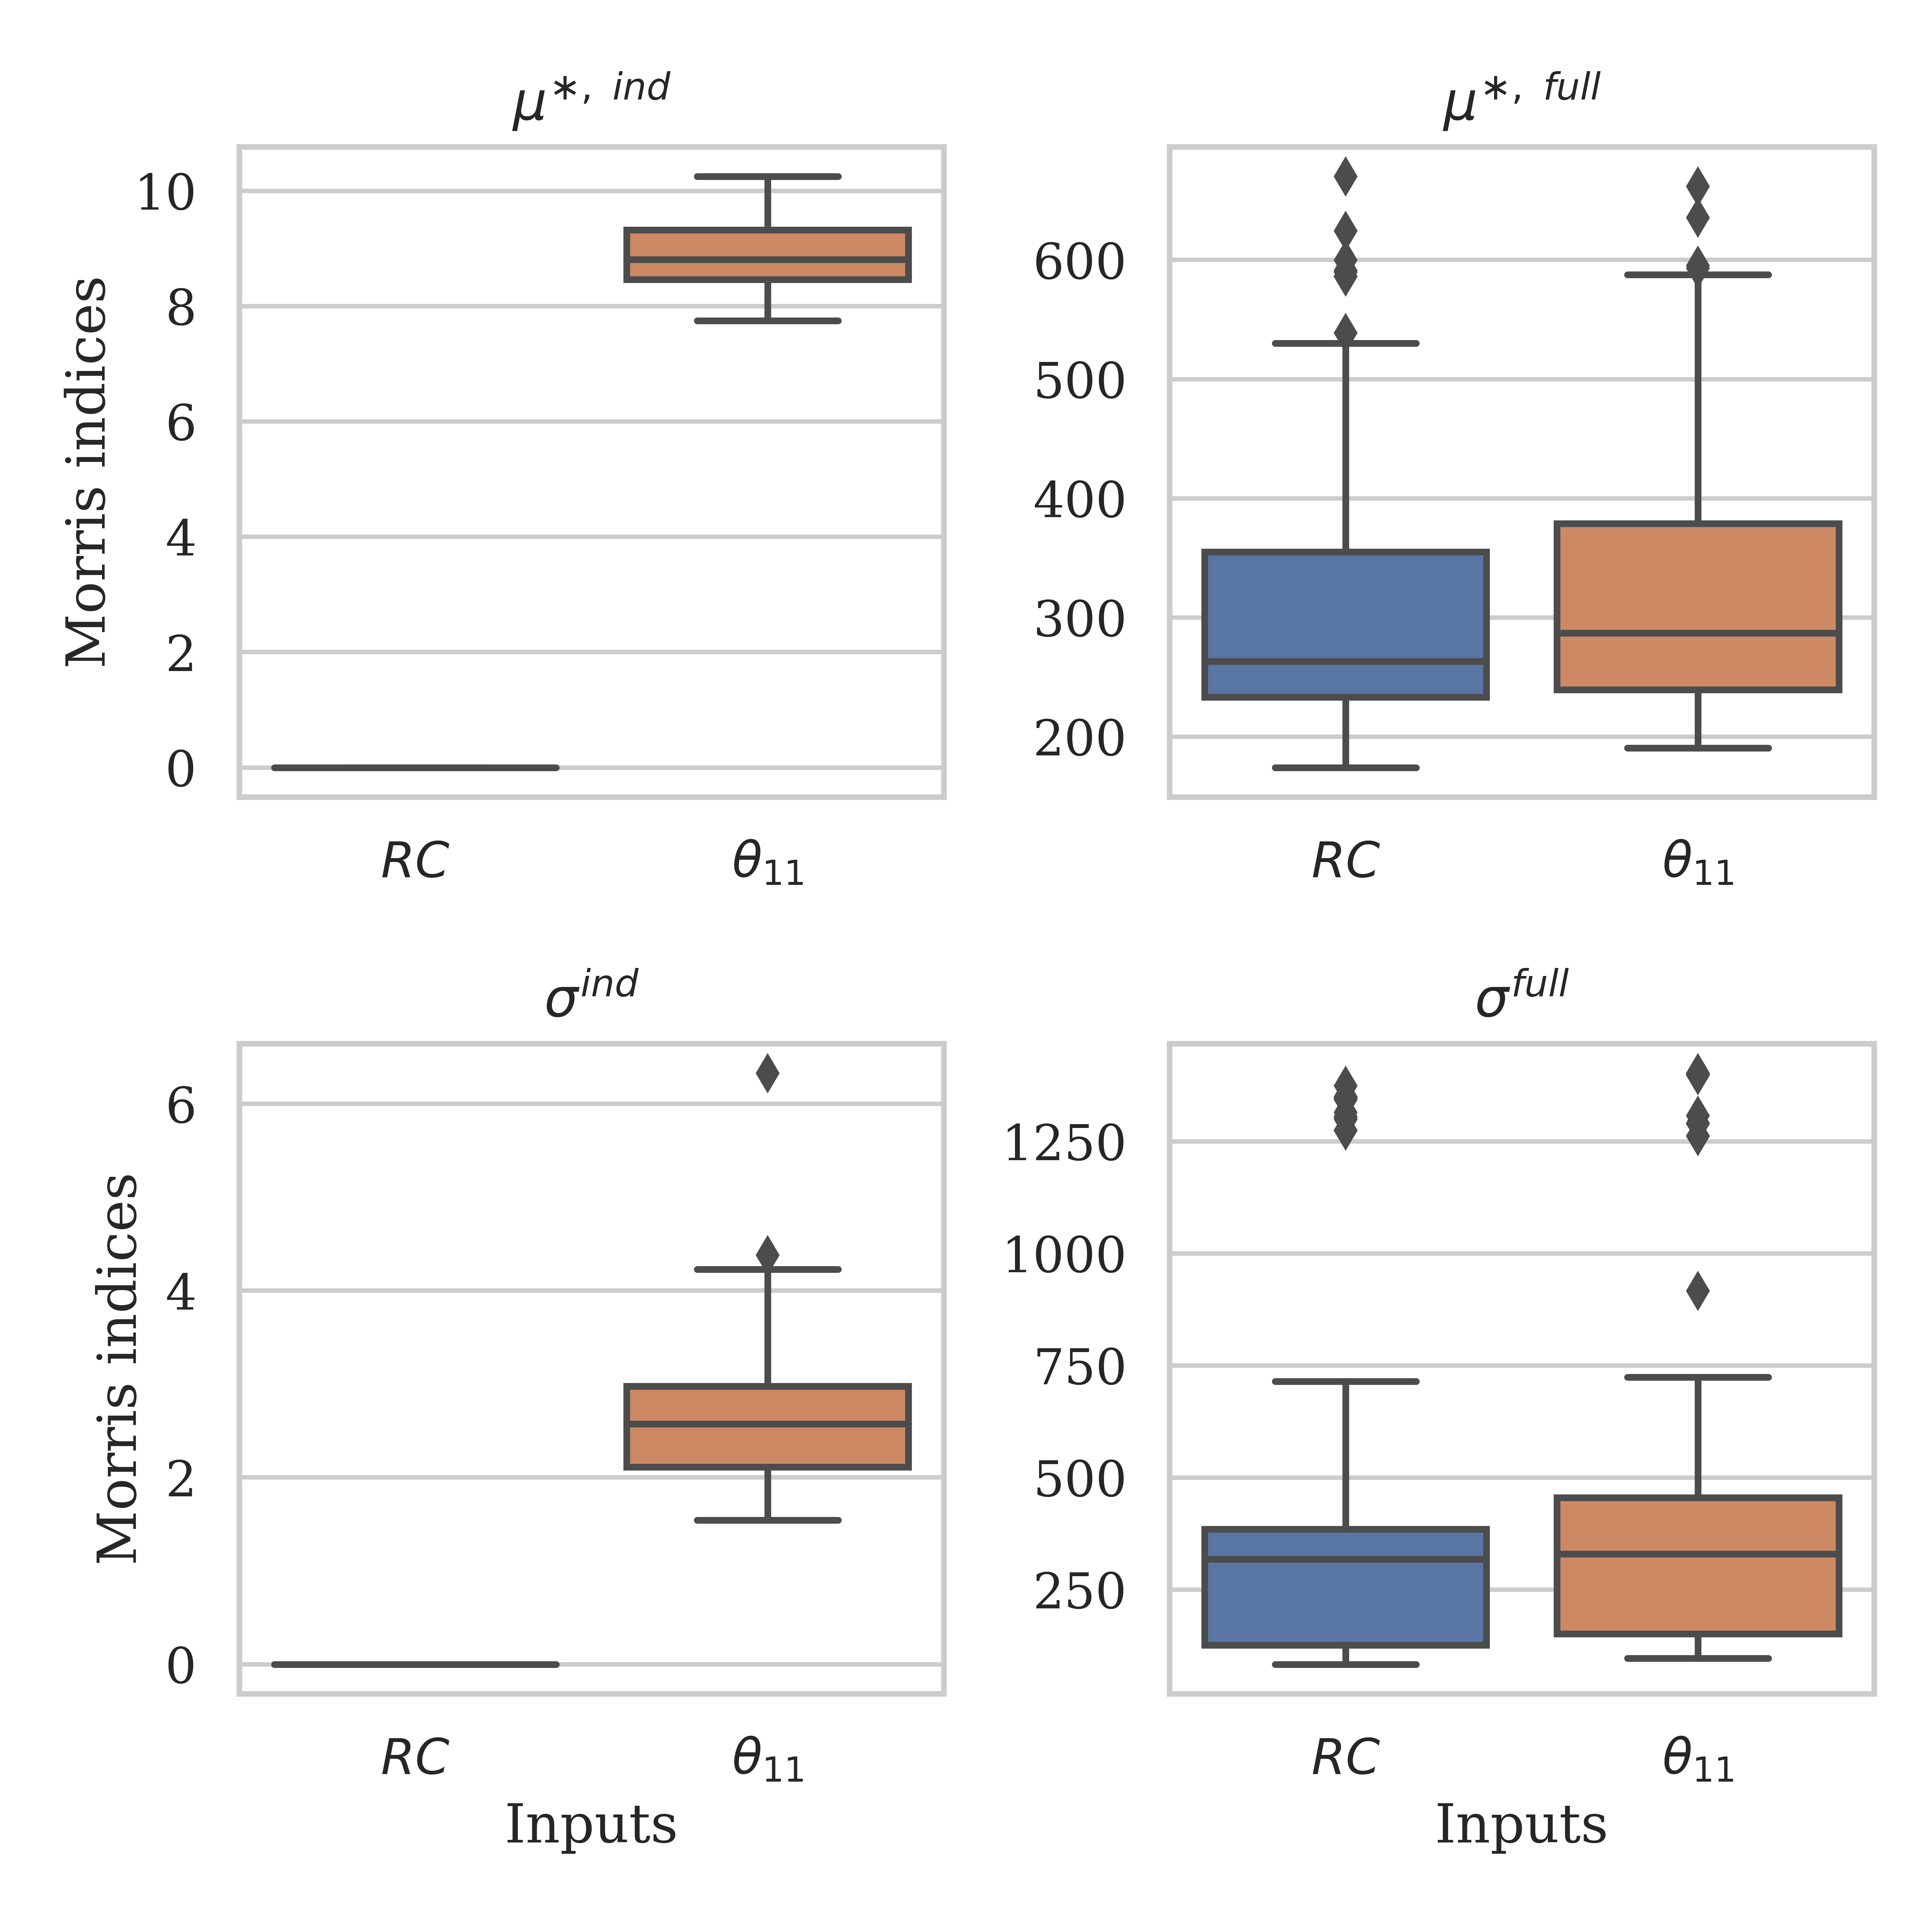
\includegraphics[scale=0.9]{../figures/boxplot_morris_replicates_100_replicates_27_draws.png}
    \end{centering}
    \end{centering}

    \small
    \textit{Notes:} Boxplots of the four Morris indices for the model inputs $RC$ and $\theta_{11}$. 100 Morris indices were estimated with $N=27$. The left panel shows \textit{independent}, the right one \textit{full} Morris indices.
\end{figure}

\begin{figure}[t]
	\caption{Convergence of Morris Indices}
    \label{morris_convergence}
    \begin{centering}
	\vspace*{-4mm}
	\begin{centering}
	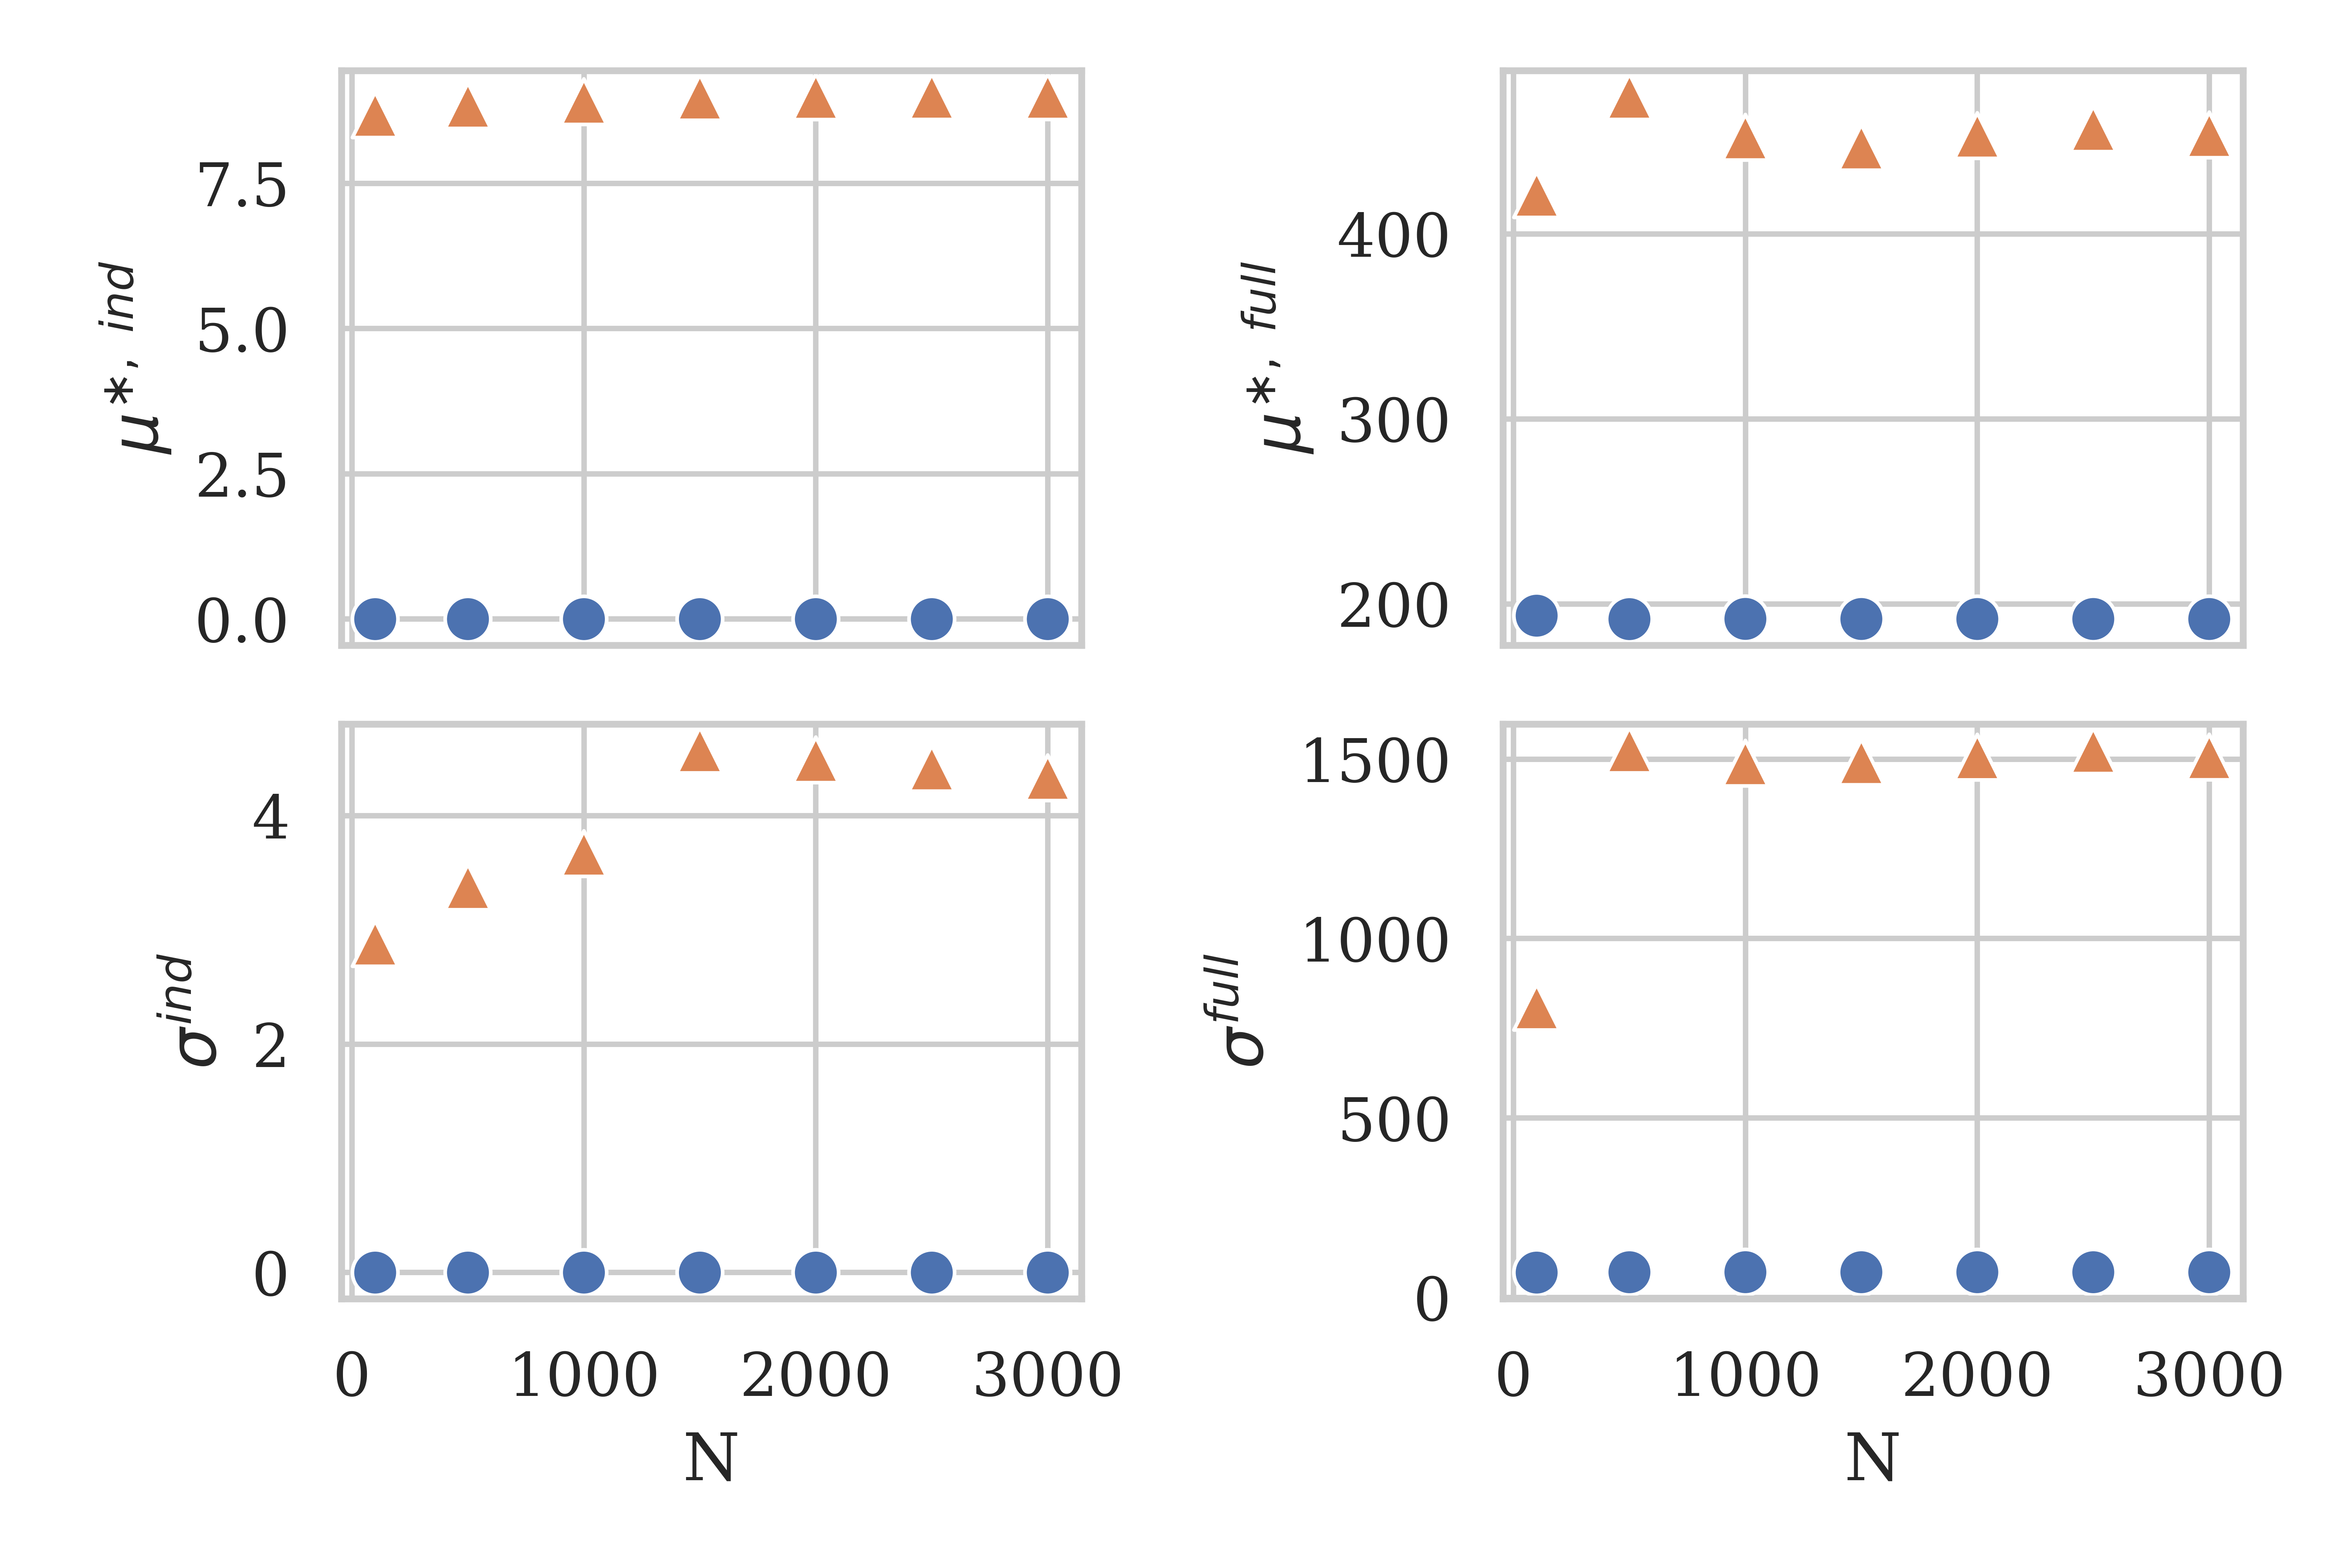
\includegraphics[scale=0.9]{../figures/morris_convergence.png}
    \end{centering}
    \end{centering}

    \small
    \textit{Notes:} Estimated Morris indices for different sample sizes $N$. The left panel shows \textit{independent} Morris indices, the right one \textit{full} Morris indices.
\end{figure}

In this section I introduce the extended Morris method for dependent samples as proposed by \citet{GM17}.

To grasp the computation procedure of the extended elementary effects, some more notation is needed. Following \citet{GM17}, let $X' = \{X_1',\ X_2',\ \dots,\ X_k'\}$ be $k$ dependent random inputs, following the joint pdf $g(X)$. Thus, $X'$ is just a set of inputs independently drawn from the set $X$. Input subsets denoted by $\bar{X}$ are conditionally drawn inputs. Hence, let $\bar{X_{-i}'}$ follow the conditional pdf $g(\bar{X_{-i}'} \mid X_{-i})$. That is $\bar{X_{-i}'}$ is drawn conditionally on the inputs in the first set $X_{-i}$. The input denoted by $\bar{X_{-i}}$ is conditionally drawn following the pdf $g(\bar{X_{-i}} \mid X_i')$. % Hence, $\bar{X_{-i}'}$ and $\bar{X_{-i}}$ differ by [].

Analogously to the independent and full Sobol' indices \citep{MTA15}, \citet{GM17} developed the following elementary effects for dependent inputs.
\begin{align}
EE_i^{ind} = \frac{f(\bar{x_i}',\ x_{-i}) - f(x_i,\ x_{-i})}{\Delta},\\
EE_i^{full} = \frac{f(x_i',\ \bar{x_{-i}}) - f(x_i,\ x_{-i})}{\Delta},
\end{align}

\noindent where
\begin{itemize}
\item $EE_i^{ind}$ denotes \textit{independent} elementary effects for input $i$, effects that exclude the contributions attributable to the dependence between input $X_i$ and $X_j$ for $i \neq j$, and
\item $EE_i^{full}$ denotes \textit{full} elementary effects for input $i$, that include the effects due to correlation with other inputs.
\end{itemize}

As in the case of the classic Morris method, the sensitivity measures for input $i$ are derived by considering $N$ random samples yielding $2 N$ elementary effects, once for the independent and once for the full elementary effects. \citet{GM17} compute the corresponding sensitivity measures as shown in \cref{mu} and \cref{sigma}. Since two sets of elementary effects are computed, they end up with a set of four sensitivity measures, $(\mu^{\ast ind}_i,\ \sigma_i^{ind})$ and $(\mu^{\ast full}_i,\ \sigma_i^{full})$.

Interpretation-wise, $X_i$ is an unimportant input if all sensitivity measures are essentially zero. If $\mu^{\ast ind}_i$ is strongly larger than zero and $\sigma_i^{ind}$ is close to zero, input $X_i$ is an important input due to its own, isolated contribution. When all sensitivity measures except $\mu^{\ast full}_i$ are close to zero, $X_i$'s contribution is due to the dependence with other important inputs. Strong interaction effects are present if either or both of the two $\sigma$'s are larger than zero \citep{GM17}.

The computation of the extended Morris indices requires the generation of dependent samples. According to \citet{GM17}, the computation involves the following steps:

\begin{enumerate}
    \item Create independent, uniformly distributed samples.
    \item Transform these uniformly distributed samples into dependent samples of a target distribution.
    \item Use the above methods for the computation of the extended elementary effects.
    \item As in the case of the classic Morris method, average over all $N$ elementary effects per input $i$ and compute their standard deviation. Do so for the \textit{independent} and \textit{full} elementary effects.
\end{enumerate}

In what follows I stick to the version of the algorithm as implemented in the \textit{econsa} Python-package \citep{OSE21}. There, the radial design is used for obtaining independent samples. To derive dependent samples, the inverse Nataf transformation is applied. The total computational cost amounts to $3kN$ model runs.

\subsection{Morris Indices for the Rust Model} \label{morris_rust_model}

\begin{table}[t]
    \caption{Relative Difference Morris Indices}
    \label{rel_diff_morris}
    \centering

    \begin{threeparttable}
        \begin{centering}
            \begin{tabular}{lrrrrrr}
\toprule
{} &   500  &  1000 &   1500 &  2000 &  2500 &  3000 \\
\midrule
$\mu_{\theta_{11}}^{\ast,\ ind}$  &   1.81 &  0.77 &   0.81 &  0.14 &  0.02 & -0.01 \\
$\sigma_{\theta_{11}}^{ind}$      &  17.18 &  8.65 &  24.70 & -1.86 & -1.66 & -1.87 \\
$\mu_{RC}^{\ast,\ ind}$           &   0.00 &  0.00 &   0.00 &  0.00 &  0.00 &  0.00 \\
$\sigma_{RC}^{ind}$               &   0.00 &  0.00 &   0.00 &  0.00 &  0.00 &  0.00 \\
$\mu_{\theta_{11}}^{\ast,\ full}$ &  12.58 & -4.63 &  -1.21 &  1.43 &  0.80 & -0.72 \\
$\sigma_{\theta_{11}}^{full}$     &  88.52 & -2.38 &   0.21 &  0.91 &  1.18 & -1.15 \\
$\mu_{RC}^{\ast,\ full}$          &  -0.96 &  0.06 &  -0.02 & -0.01 &  0.01 & -0.01 \\
$\sigma_{RC}^{full}$              &   1.42 &  0.18 &  -0.10 & -0.01 & -0.03 &  0.04 \\
\bottomrule
\end{tabular}

            \begin{tablenotes}
                \small
                \item \textit{Notes:} The percentage difference between Morris indices for different values of $N$. For example, for $\mu^{\ast,\ full}$ Percentage changes are calculated by $\frac{\mu^{\ast,\ full,\ n-1}_i - \mu^{\ast,\ full,\ n}_i}{\mu^{\ast,\ full,\ n}_i}$, for $i \in \{RC,\ \theta_{11}\}$ and $n$ denoting the different values of $N$.
            \end{tablenotes}
        \end{centering}

        \end{threeparttable}
\end{table}

Similar to the procedure described in \cref{comp_shap}, I estimate Morris indices in two different ways: Firstly, I estimate 100 replicates for a relatively low sample size to get a sense of the variability in estimates, Then, I consecutively increase the sample size to investigate
the estimation procedure further. Uniformly distributed samples are drawn from a Sobol'
sequence \citep{S76}.\footnote{The Sobol' sequence is a quasi-random sequence used for Quasi-Monte Carlo methods. \citet{KTA12} argue that Quasi-Monte Carlo estimators converge faster than estimators based on pseudo-random numbers.}

Firstly, I estimate 100 sets of Morris indices. In order to ensure comparability to the Shapley effects , I use the same total computational cost as for the data used for \cref{boxplot_shapley}. I set $N = 27$, which amounts
to a total cost of 162 model evaluations, which differs slightly from the computational
cost of the Shapley effects (160) because of rounding.\footnote{The same computational cost as for Shapley effects is achieved by solving $6 \cdot N = 160 \Leftrightarrow N = \frac{160}{6} \approx 26.67$.} As stated above, there are four different
sensitivity indices estimated: $(\mu^{\ast ind}_i,\ \sigma_i^{ind})$ and $(\mu^{\ast full}_i,\ \sigma_i^{full})$. The distribution of the
estimated Morris indices is given in \cref{morris_replicates}.

Analysing \cref{morris_replicates}, we can get a sense of the uncertainty inherent in the estimation procedure,
given the admittedly small sample size. For the independent Morris indices, there exists a
very clear ranking: both values indicate that $RC$ is uninfluential. For $\theta_{11}$ the situation is
different: both independent indices, $(\mu^{\ast ind}_{\theta_{11}},\ \sigma_{\theta_{11}}^{ind})$, are nonzero. Surprisingly, for the full Morris indices,
we fail to observe a clear input ranking. Estimates of $(\mu^{\ast full}_i,\ \sigma_i^{full})$ are very volatile, but
clearly different from zero. Seemingly, no
clear input ranking is achieved. However, Morris indices were primarily developed to
identify non-influential inputs. Both inputs are important if the full Morris indices are
considered.

To investigate whether the individual pairs of full Morris indices, $(\mu^{\ast full}_i,\ \sigma_i^{full})$, for the
two inputs $i \in \{RC,\ \theta_{11}\}$ yield the correct input ranking, I simply compare their values
per replicate. Details are given in \cref{accuracy}. Surprisingly, only about 60 of the 100 replicates yield the correct importance ranking
for $\mu^{\ast full}_i$. I conclude that ranking based on full Morris indices in the case of the Rust model can be misleading given the small sample size.
The influence of dependence seems to be so large that indices cannot be ranked according to their full variance contribution.

\begin{table}[t]
    \centering
    \caption{Morris Indices for $N=3\,000$}
    \label{morris_3000}
    \begin{threeparttable}
    \begin{centering}
        \begin{tabular}{llrr}
\toprule
     &               &  $\mu^\ast$ &  $\sigma$ \\
Type & Input &             &           \\
\midrule
independent & $RC$ &        0.00 &      0.00 \\
     & $\theta_{11}$ &        8.99 &      4.33 \\
full & $RC$ &      191.82 &     70.88 \\
     & $\theta_{11}$ &      453.59 &   1505.77 \\
\bottomrule
\end{tabular}

        \begin{tablenotes}
            \small
            \item \textit{Notes:} \textit{Independent} and \textit{full} Morris indices for $RC$ and $\theta_{11}$ using $N=3\,000$.
        \end{tablenotes}
    \end{centering}

    \end{threeparttable}

\end{table}

Secondly, I compute Morris indices for a set of number of draws. I consider $N \in \{100,\ 500,\ 1000,\ 1500,\ 2000,\ 2500,\ 3000\}$. The corresponding results are shown in \cref{morris_convergence}. The obtained Morris indices clearly confirm the input ranking implied by the Shapley effects for both, $\mu^{\ast ind}_i$ and $\mu^{\ast full}_i$. Further, Morris indices
seem to converge as $N$ increases. In \Cref{rel_diff_morris} specific information on the convergence behaviour is provided. \citet{ASAV19} show for the classical (independent) Morris indices that they do indeed converge with increasing sample size. Since in the end, the full Morris indices are estimated in a similar fashion, similar behaviour for full indices is expected. However, \textit{full} Morris indices do not converge for all replicates as seen in \cref{morris_replicates} and supported further by the results in \cref{accuracy}. In fact, the share of correct rankings steadily declines as $N$ increases. Intrigued by this result, I investigate whether this behaviour can be observed for a larger sample size as well.To that end, I consider the replicate of Morris indices with $N=500$ which shows the largest difference $\mu^{\ast,\ full}_{RC} - \mu^{\ast,\ full}_{\theta_{11}}$ and re-estimate the full indices for larger sample sizes, i.e. for $N \in \{3\,000,\ 4\,000,\ 6\,000,\ 8\,000\}$. Details are shown in \cref{appendix_morris_seed_67} in Appendix A. There, Morris indices seem to converge, but still yield the wrong input ranking. Unfortunately, due to the computational limitations I face, I cannot investigate this further.
% Although Morris indices are volatile, \citet{GM17} point out that a high estimation precision is not necessarily needed as long as the identification of uninfluential inputs is achieved.

Let us inspect the Morris indices for $N = 3\,000$ in more detail. Consult \cref{morris_3000} for the
resulting sensitivity indices. The computational cost for this value of $N$ amounts to $18\,000$
model evaluations. As in the other trials, \cref{morris_3000} shows $(\mu^{\ast ind}_{RC},\ \sigma_{RC}^{ind})$ equal to zero.
If only the independent Morris indices are considered, we erroneously
conclude that input $RC$ is a non-influential input by neglecting the variance contribution due to dependence. Since none of the inputs exhibits $(\mu^{\ast ind}_i,\ \sigma_i^{ind})$ and $(\mu^{\ast full}_i,\ \sigma_i^{full})$ close to zero at the same time, both inputs have to be considered as influential ones and thus cannot be fixed without influencing the output.
Since both independent indices for $\theta_{11}$, $(\mu^{\ast ind}_{\theta_{11}},\ \sigma_{\theta_{11}}^{ind})$, are high, there are either strong interaction and/or non-linear effects present.
% Since independent sensitivity indices for $RC$ are both zero, the reason for the high $\sigma_{\theta_{11}}^{ind}$ must be driven by the presence of non-linear effects in $\theta_{11}$. Regarding the model structure we can conclude that there are no interaction effects between $RC$ and $\theta_{11}$.